\chapter{実装}\label{cha:Implementation}
本章では、本研究で試作したモータ特性表自動生成ツールの実装について説明する。\\
% 本章では、本研究で試作したモータ特性表自動生成ツールの機能である、「モータ特性表生成機能」、「ツールの実行機能」、「エラー表示機能」の実装について説明する。\\
% \section{特性表生成機能}\label{tokuseihyou_seisei}
% モータ特性表自動生成ツールの処理の流れを図\ref{fig:syori}に示す。\\
% \begin{figure}[t]
% 	\centering
% 	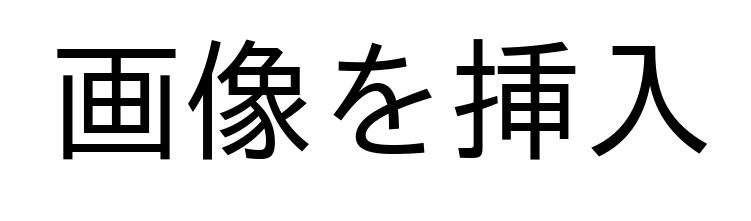
\includegraphics[width=16.5cm,height=10cm]{./Image/sample.png}
% 	\caption{モータ特性表自動生成ツールの処理の流れ}
% 	\label{fig:syori}
%   \end{figure}
% \section{モータ特性表生成機能}\label{tokuseisei}
モータ特性表自動生成機能の処理の流れを以下に示す。
\begin{enumerate}
    \item 実行コマンドを取得する
    \item 第1引数で指定されたcsvファイルを読み込む
    \item 第2引数、第3引数で指定したモジュール名が持つデータを、csvファイルから取得する
    \item モータ特性表の各要素を算出する
    \item 特性表を作成する
    \item 特性グラフを作成する
    \item モータ特性表を生成する
\end{enumerate}

以下、各処理について具体的に説明する。

\section{実行コマンドの引数の取得}\label{comandget}
この処理では、Pythonスクリプトに渡されたコマンドライン引数のリストであるsys.argvで引数を取得し、エラーの検出を行う。
処理の流れを以下に示す。
\begin{enumerate}
    \item sys.argvの要素数を取得する
    \item 要素数が4以外であれば、図\ref{fig:error_hikisuu}のエラーを表示する
    \item sys.argvの1番目のデータを、ファイル名を保存するために用意した変数に格納する
\end{enumerate}

\section{csvファイルの読み込み}\label{csvfairu}
Pythonで実装するため、Pythonの標準ライブラリのcsvモジュールをインポートし、
csvファイルを読み込む。
以下の条件の時に、オブジェクト名が間違っていると判断する。

エラーは、
以下の条件の1つにでも該当した場合、ファイル名が間違っていると判定し、エラー文を画面上に出力する。
\begin{itemize}
    \item ファイルの拡張子が「.csv」ではない
    \item ファイルを開く際にエラーが出たとき
\end{itemize}

\section{第2引数、第3引数で指定されたモジュールが持つデータを、csvファイルから取得}\label{syutoku_data}
\ref{csvfairu}節で読み込んだcsvファイルから、以下のデータを取得する。

\begin{itemize}
    \item 電流
    \item 電圧
    \item トルク
    \item 角速度
\end{itemize}

\ref{OM}節で述べたように、OpenModelicaから出力されたcsvファイルの1行目には、
各部品のモジュール名を含んだ変数名が記載されている。これを利用して、次の処理で必要なデータを取得する。

\begin{enumerate}
    \item 取得したいデータを持つ変数名を検索する
    \item 変数名のある場所の添字を取得する
    \item 各データごとに用意した配列に、にある値を格納する
    \item 
    \item あ
    \item csvファイルが読み終わるまでーーの処理を繰り返し行う
\end{enumerate}
!!!取得したいデータを持つ変数名を探し、その変数名がある場所の添字を取得する。
各データごとに用意した配列に、同じ添字の位置にある値を繰り返し処理で格納する方法でそれぞれの値を取得する。
アルゴリズムっぽく


以下の条件の1つにでも該当した場合、指定したオブジェクト名が間違っていると判定し、エラー文を画面上に出力する。
\begin{itemize}
    \item 電流値のある添え字を持つ変数が、初期値である「0」であった場合
    \item 電圧のある添え字を持つ変数が、初期値である「0」であった場合
    \item トルクのある添え字を持つ変数が、初期値である「0」であった場合
    \item 角速度のある添え字を持つ変数が、初期値である「0」であった場合
\end{itemize}

\section{モータ特性表の各要素を算出する}\label{keisan}
\ref{syutoku_data}節で取得したデータを用いて、\ref{kenkyu_mokuteki}節で挙げた各要素の値を求める。

\subsection{電圧}\label{sub:keisan_dennatu}
% シミュレーション時に印加した値を取る。
今回試作したツールでは、電源部品の電圧値を電圧とする。

\subsection{始動電流}\label{sub:keisan_sidouden}
% 始動電流とは、モータの起動時に流れる大きな電流のことである。
% モータが起動した後はモータ自体が発電機にもなり、逆起電力を発生するため、モータ・コイル部分にかかる電圧が下がり、電流値も下がる。
% したがって、電流値の配列の中で一番大きい値を始動電流とする。
モータが起動した後は、逆起電力を発生させるため、モータ・コイル部分にかかる電圧が下がり、電流値も下がる。\\
したがって、今回試作したツールでは、電流値の中で一番大きい値を始動電流とする。
% https://www.tsugawa.co.jp/glossary/ 

\subsection{停動トルク}\label{sub:keisan_teidoutoruku}
% 停動トルクとは、モータが出しうる最大トルクで、このトルク以上の負荷がかかれば、モータは停止する値となる。
% したがって、トルク値の配列の中で一番大きい値を停動トルクとする。
したがって、今回試作したツールでは、トルク値の中で一番大きい値を停動トルクとする。

% https://www.orientalmotor.co.jp/tech/glossary/ta11/

\subsection{最大効率}\label{sub:keisan_saidaikouritu}
効率は以下の式で算出する。

\[
    \mbox{効率} = \frac{\mbox{出力}}{\mbox{入力}}  * 100 
\]
\[
    \mbox{出力} = \mbox{角速度} * \mbox{トルク} 
\]
\[  
    \mbox{入力} = \mbox{電圧} * \mbox{電流} 
\]

今回試作したツールでは、効率値の中で一番大きい値を最大効率とする。


% https://www.jp-igarashi.com/product/product_motors/curve.html

\subsection{定格トルク}\label{sub:keisan_teikakutoruku}
% 最大効率時のトルクを定格トルクという。
したがって、トルク値の配列の中で、最大効率のある効率値の配列の添字と同じ位置にある値が定格トルクとなる。


% http://www.sagamimicro.co.jp/product/aboutusage.html

\subsection{定格回転数}\label{sub:keisan_teikakukaiten}
% 最大効率時の回転数を定格回転数という。
回転数は以下の式で算出できる。

\[
    \mbox{回転数} = \frac{30 * \mbox{角速度}}{\pi}   
\]

したがって、一度繰り返し処理で角速度を回転数に変換し、回転数値の配列の中で、最大効率のある効率値の配列の添字と同じ
位置にある値が定格回転数となる。

% https://mathwords.net/kaitensu

\subsection{定格電流}\label{sub:keisan_teikakuden}
% 定格電流とは、モータに定格トルクがかかっているときの電流値である。
したがって、電流値の配列の中で、定格トルクのあるトルク値の配列の添字と同じ位置にある値が定格電流となる。

% http://fa-faq.mitsubishielectric.co.jp/faq/show/18504?category_id=1937&site_domain=default

\subsection{定格出力}\label{sub:keisan_teikakusyutu}
% 定格出力とは、定格動作点における出力の値である。
定格出力は以下の式で算出できる。

\[  \mbox{定格出力} = \mbox{定格トルク} * \mbox{定格回転数} * \frac{2\pi}{60} \]
% \ref{sub:keisan_teikakukaiten}章で求めた定格回転数と\ref{sub:keisan_teidoutoruku}章で求めた定格トルクを
% http://www.nidec-servo.com/jp/digital/pdf/A_technique.pdf

\subsection{最大回転数}\label{sub:keisan_saidaikai}
今回試作したツールでは、回転数地の配列の中から一番大きい値を

\section{特性表を作成}\label{sakusei_hyou}
\ref{keisan}章で求めた各値と、\ref{kenkyu_mokuteki}章で挙げた各要素を、
電圧から順に","で区切りつつ特性表生成配列に格納する。そして特性表生成配列を用いてcsvファイルを作成する。


\section{特性グラフを作成}\label{sakusei_gura}


\section{モータ特性表を生成}\label{seisei_mort}


